\section{Gates} 
We describe gate behaviors using matrices, and then describe the effect of a gate as a transformation of the tree representing the input state.
%
We start by modeling classical digital gates in the quantum setting.
%
Then, we introduce some quantum gates and show we can represent them using matrices.

\paragraph{Classical Gates}
\begin{figure} 
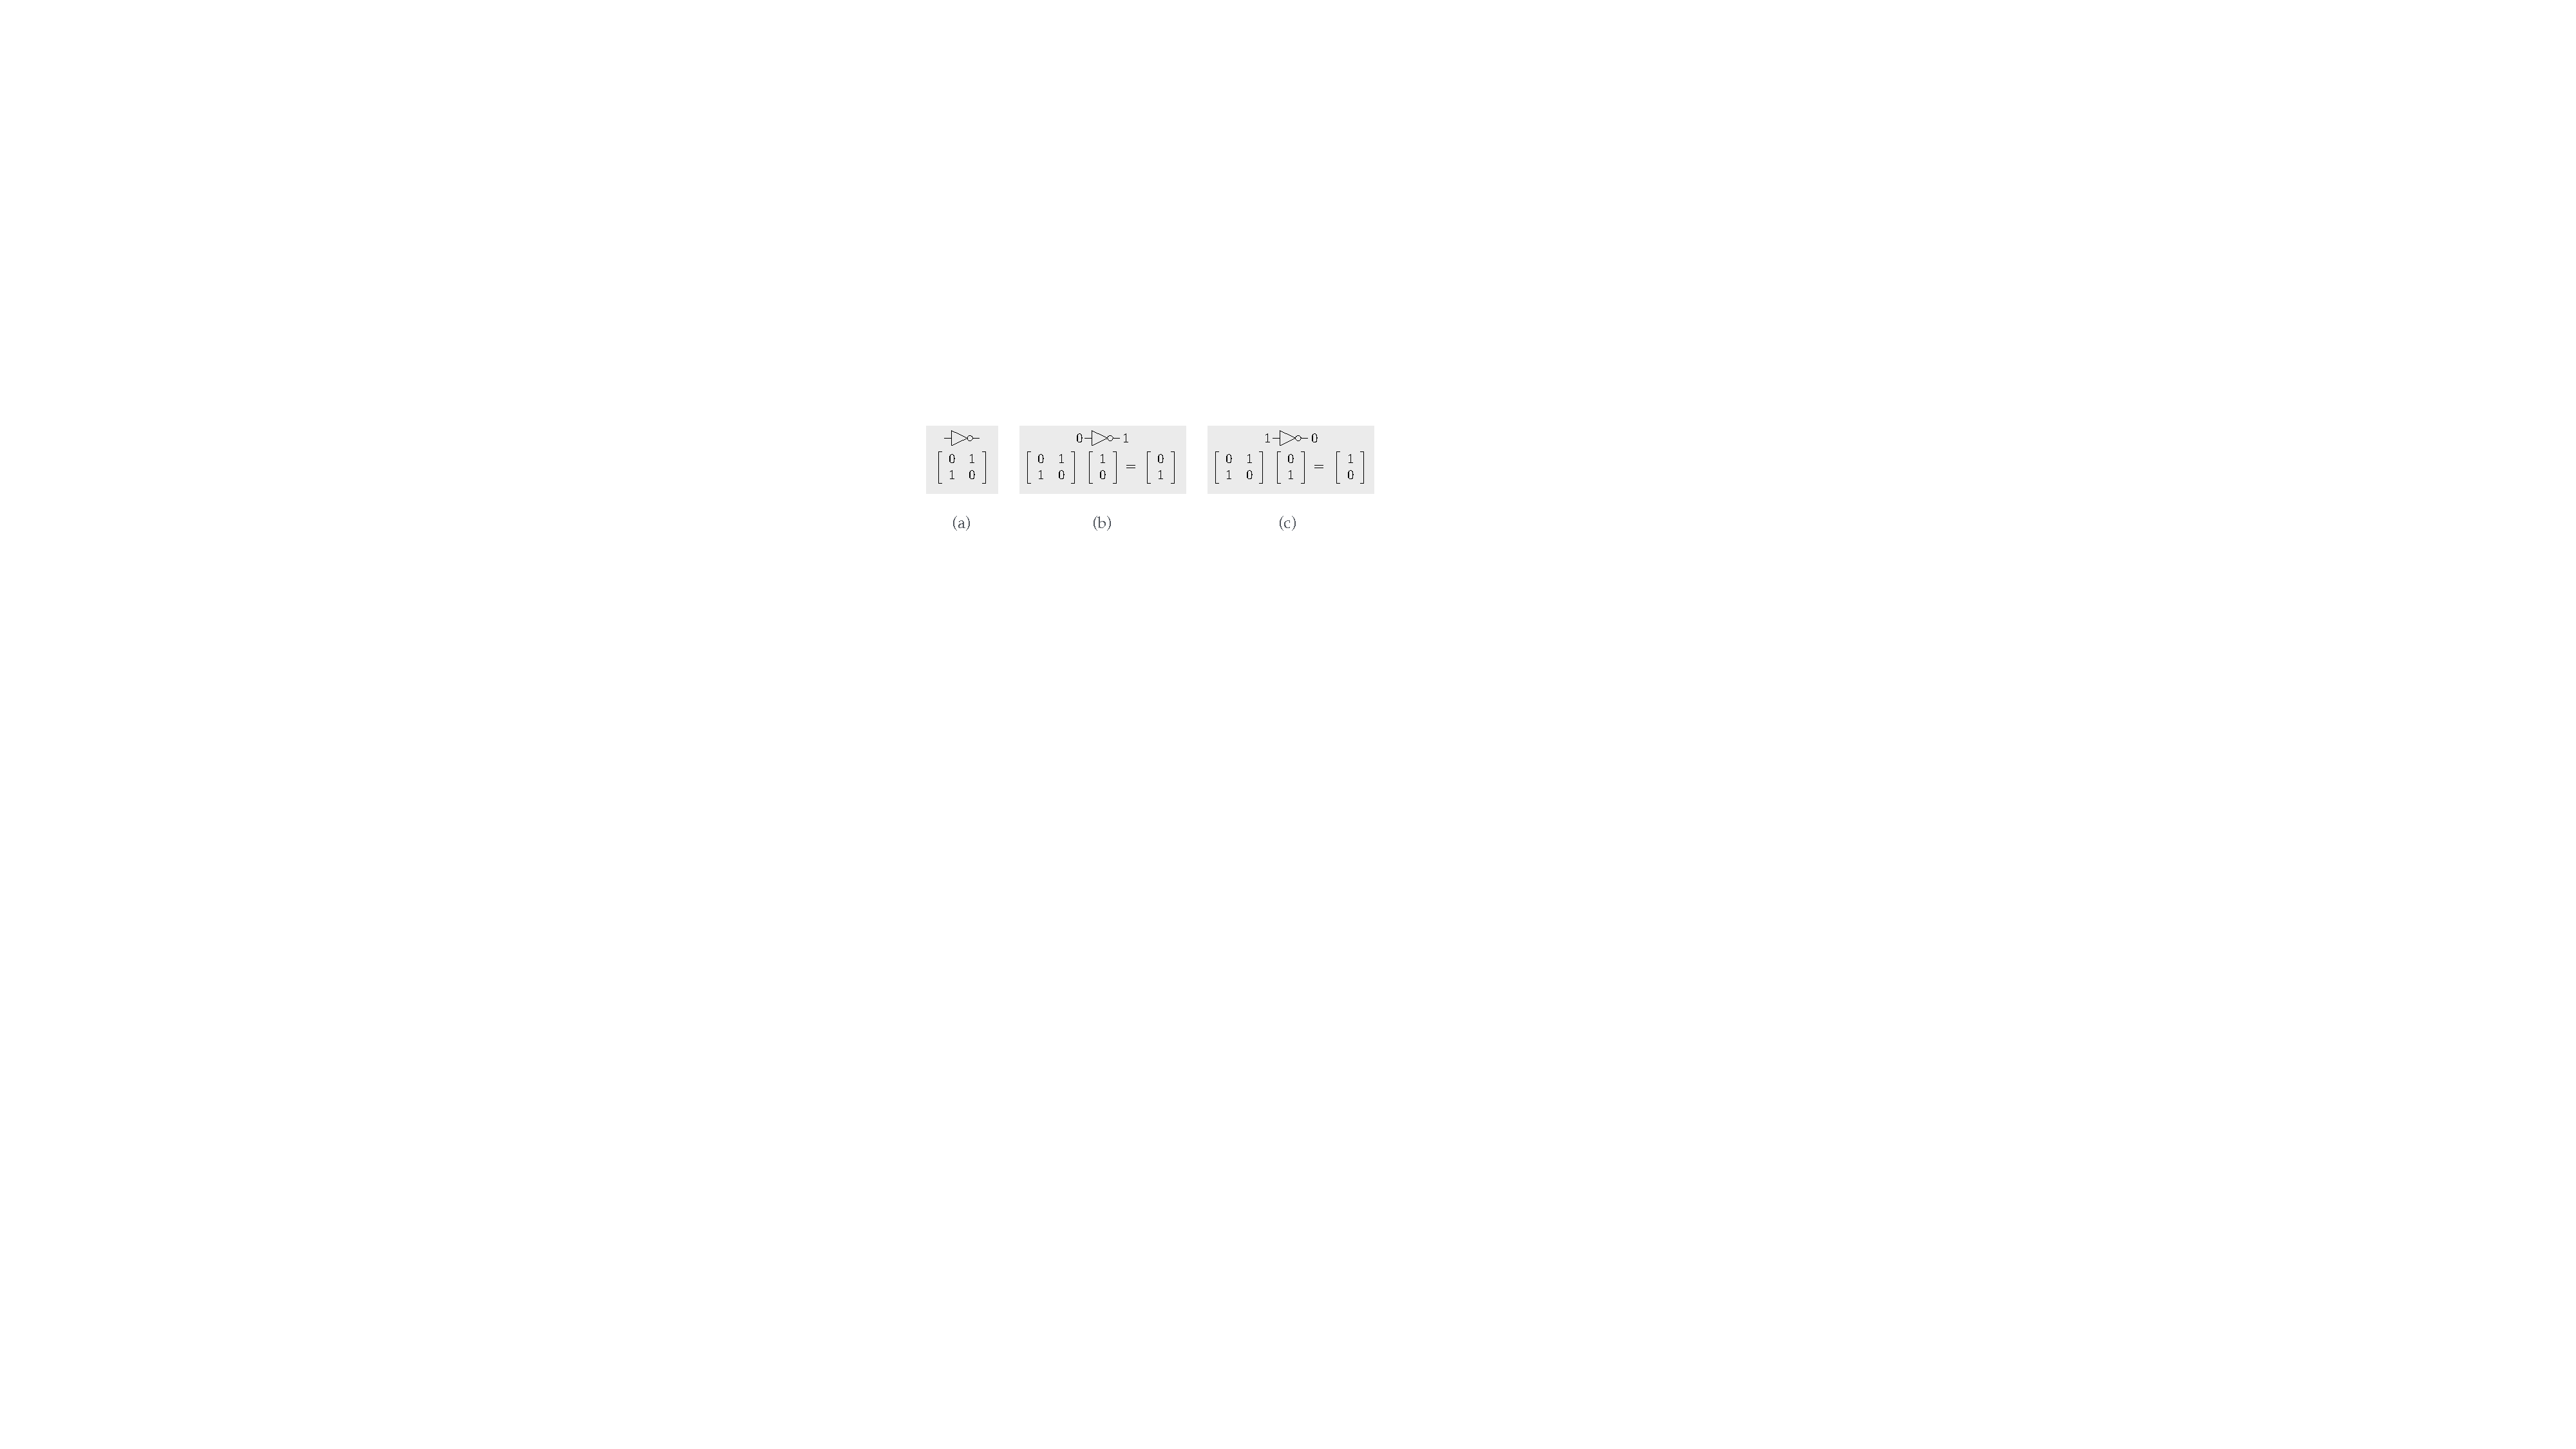
\includegraphics[]{Figures/Gates/not} 
\caption{(a) The $\notgate$ gate together with its matrix presentation.
(b) Applying the gate to $0$, represented by $[1\;\;0]^T$, will give $1$, i.e., $[0\;\;1]^T$.
(c) Applying the gate to $1$ will give $0$.}
\label{not:gate:fig}
\end{figure}
%
Logical gates, such as $\andgate$, $\orgate$, and $\notgate$, are the fundamental components of digital circuits. 
%
They take binary inputs (0s and 1s) and produce a single binary output.
%
Each type of gate implements a specific binary function, e.g., the output of an $\andgate$ gate is the conjunction of its inputs.
%
In order to prepare for quantum gates, we will represent the behavior of classical gates by matrices.
%
Let us take the $\notgate$ gate as an example (\cref{not:gate:fig}).
%
For a given (basis) state, we compute the result of applying the gate by multiplying the matrix representing the gate with the input state.
%
%
The gate has one input and one output bit, and hence its behavior is described by a $2\times2$-matrix.
%
The input and output states are both column vectors.

\begin{figure} 
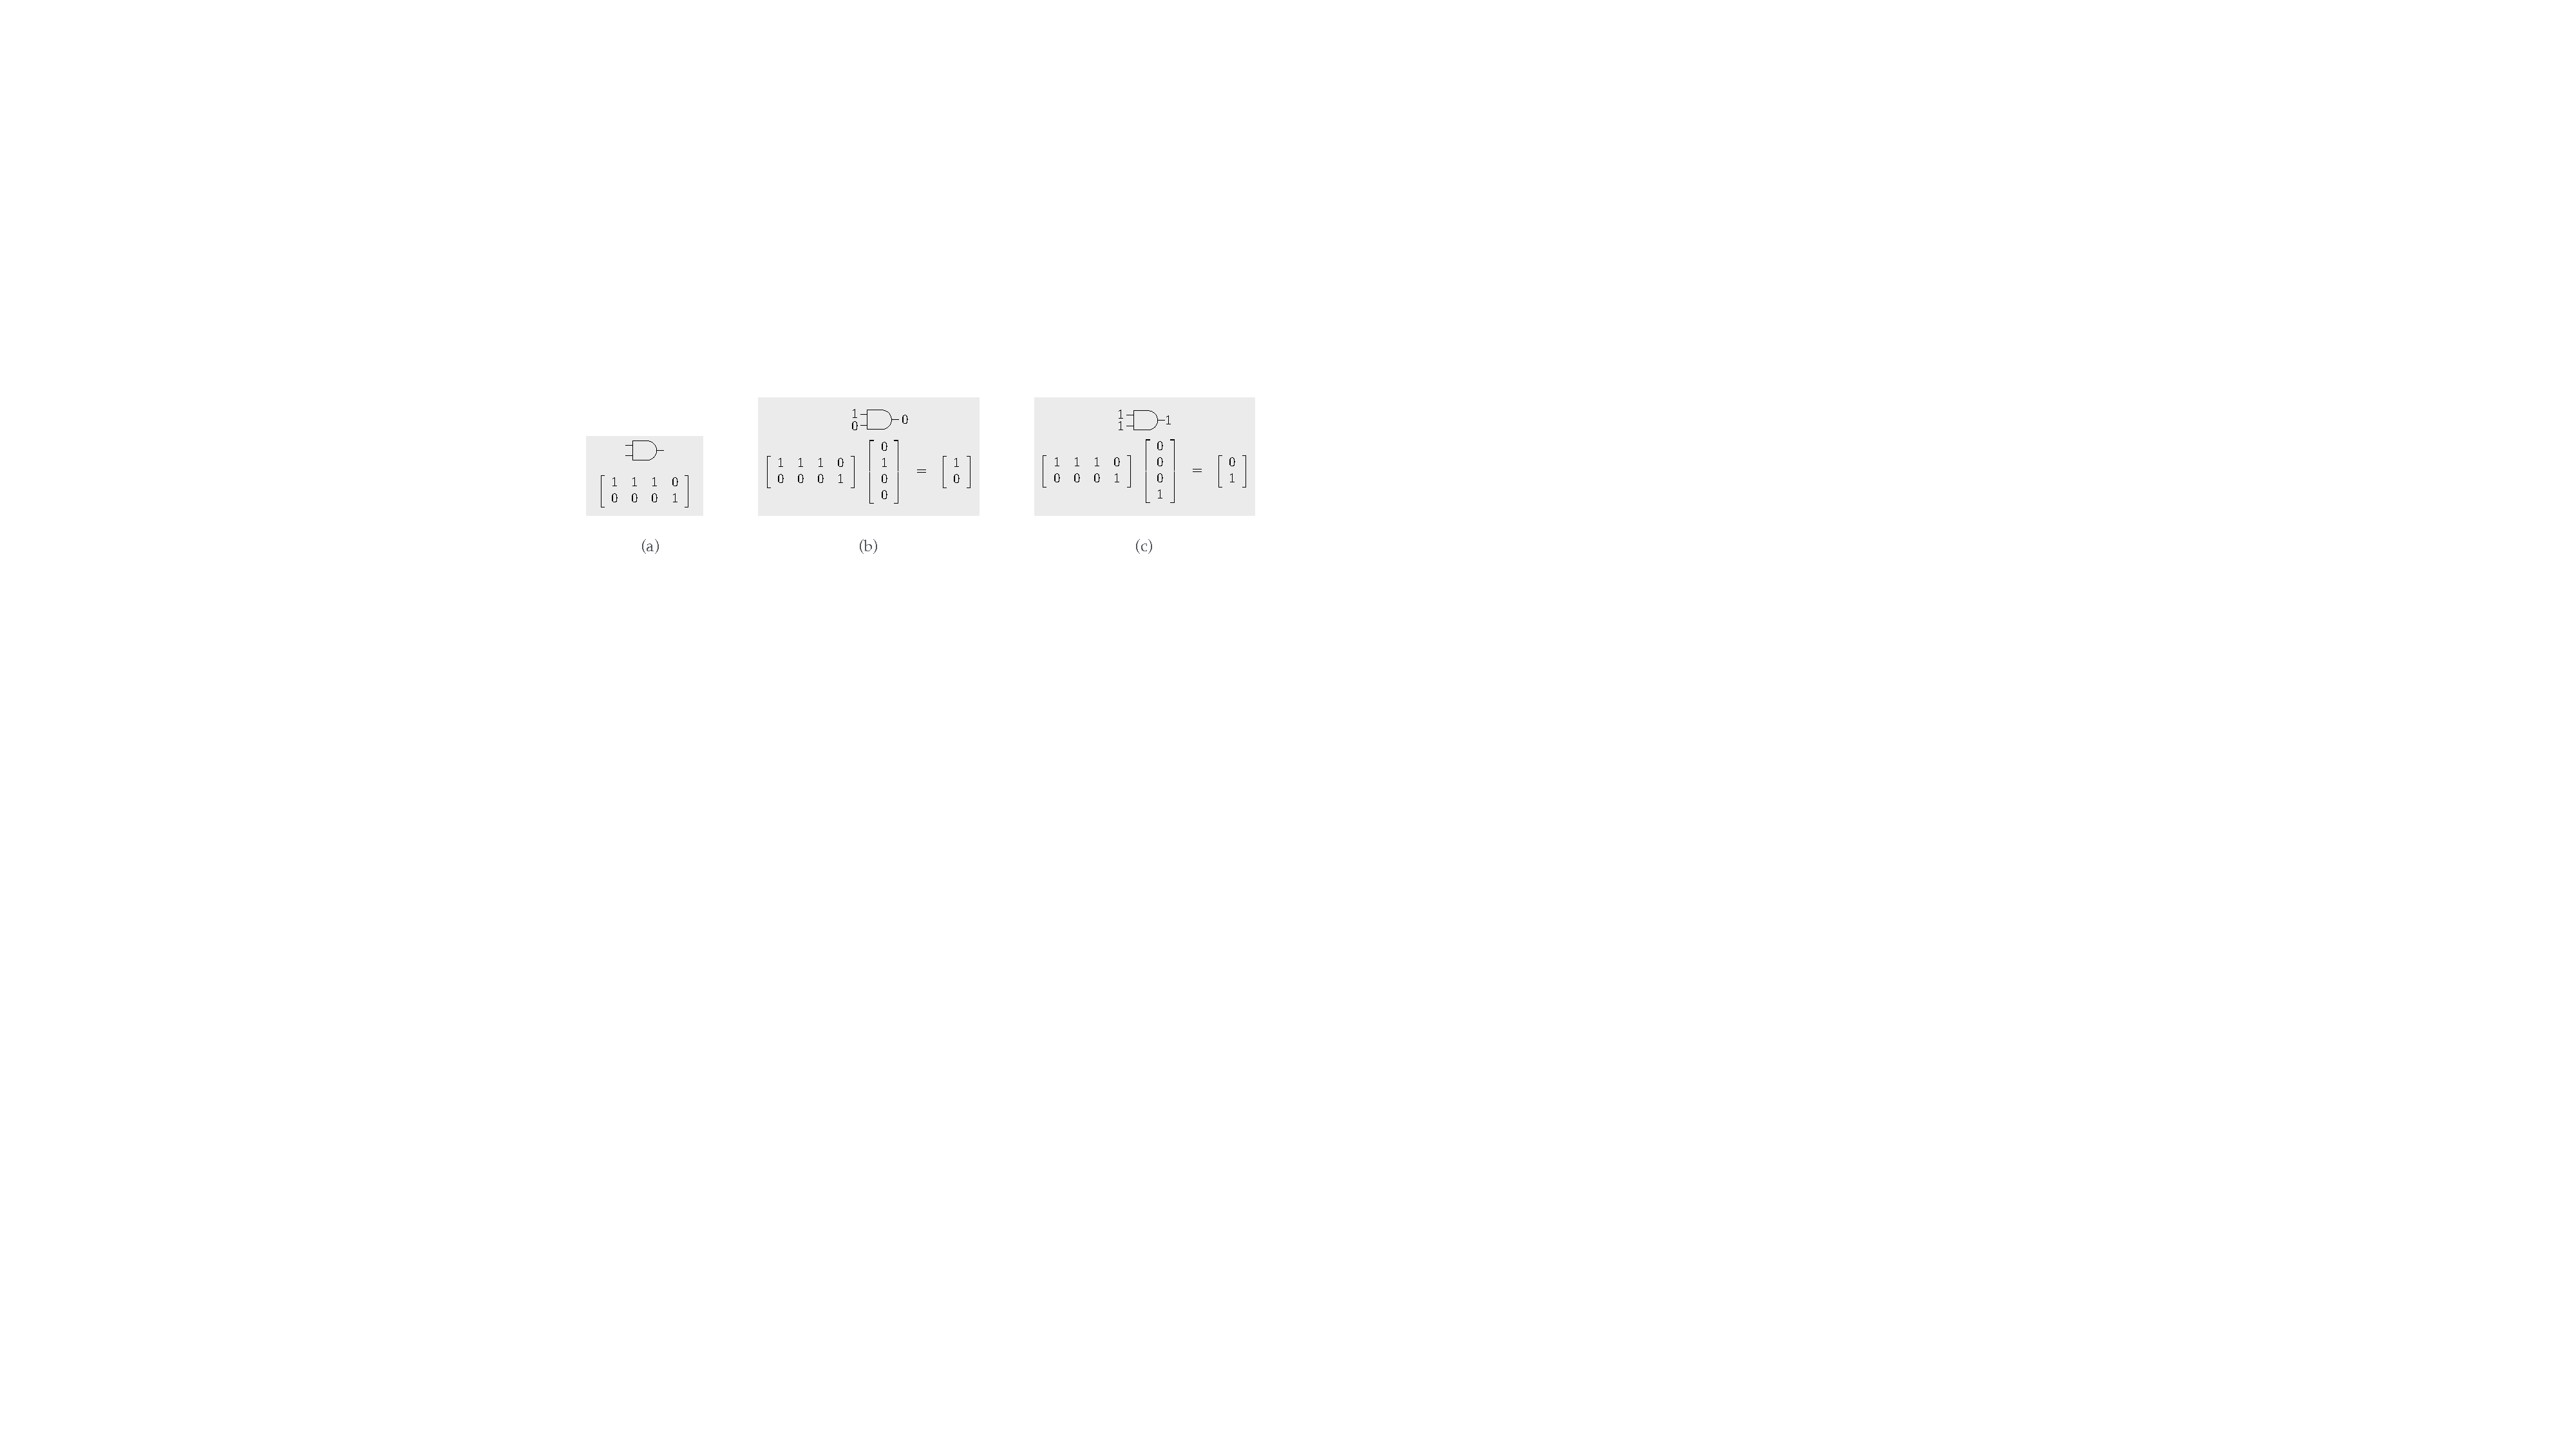
\includegraphics[scale=0.7]{Figures/Gates/and} 
\caption{(a) The {\tt AND gate} together with its matrix presentation.
(b) Applying the gate to $01$, represented by $[0\;\;1\;\;0\;\;0]^T$, will give $0$. 
(c) Applying the gate to $11$, represented by $[0\;\;0\;\;0\;\;1]^T$, will give $1$.}
\label{and:gate:fig}
\end{figure}
%
\cref{and:gate:fig} depicts the $\andgate$ gate.
%
The gate has two input bits and one output bit, and hence its behavior is described by a $2\times4$-matrix.
%
The input state is of length $4$ and the output state has length $2$.

\paragraph{Quantum Gates}
\begin{figure} 
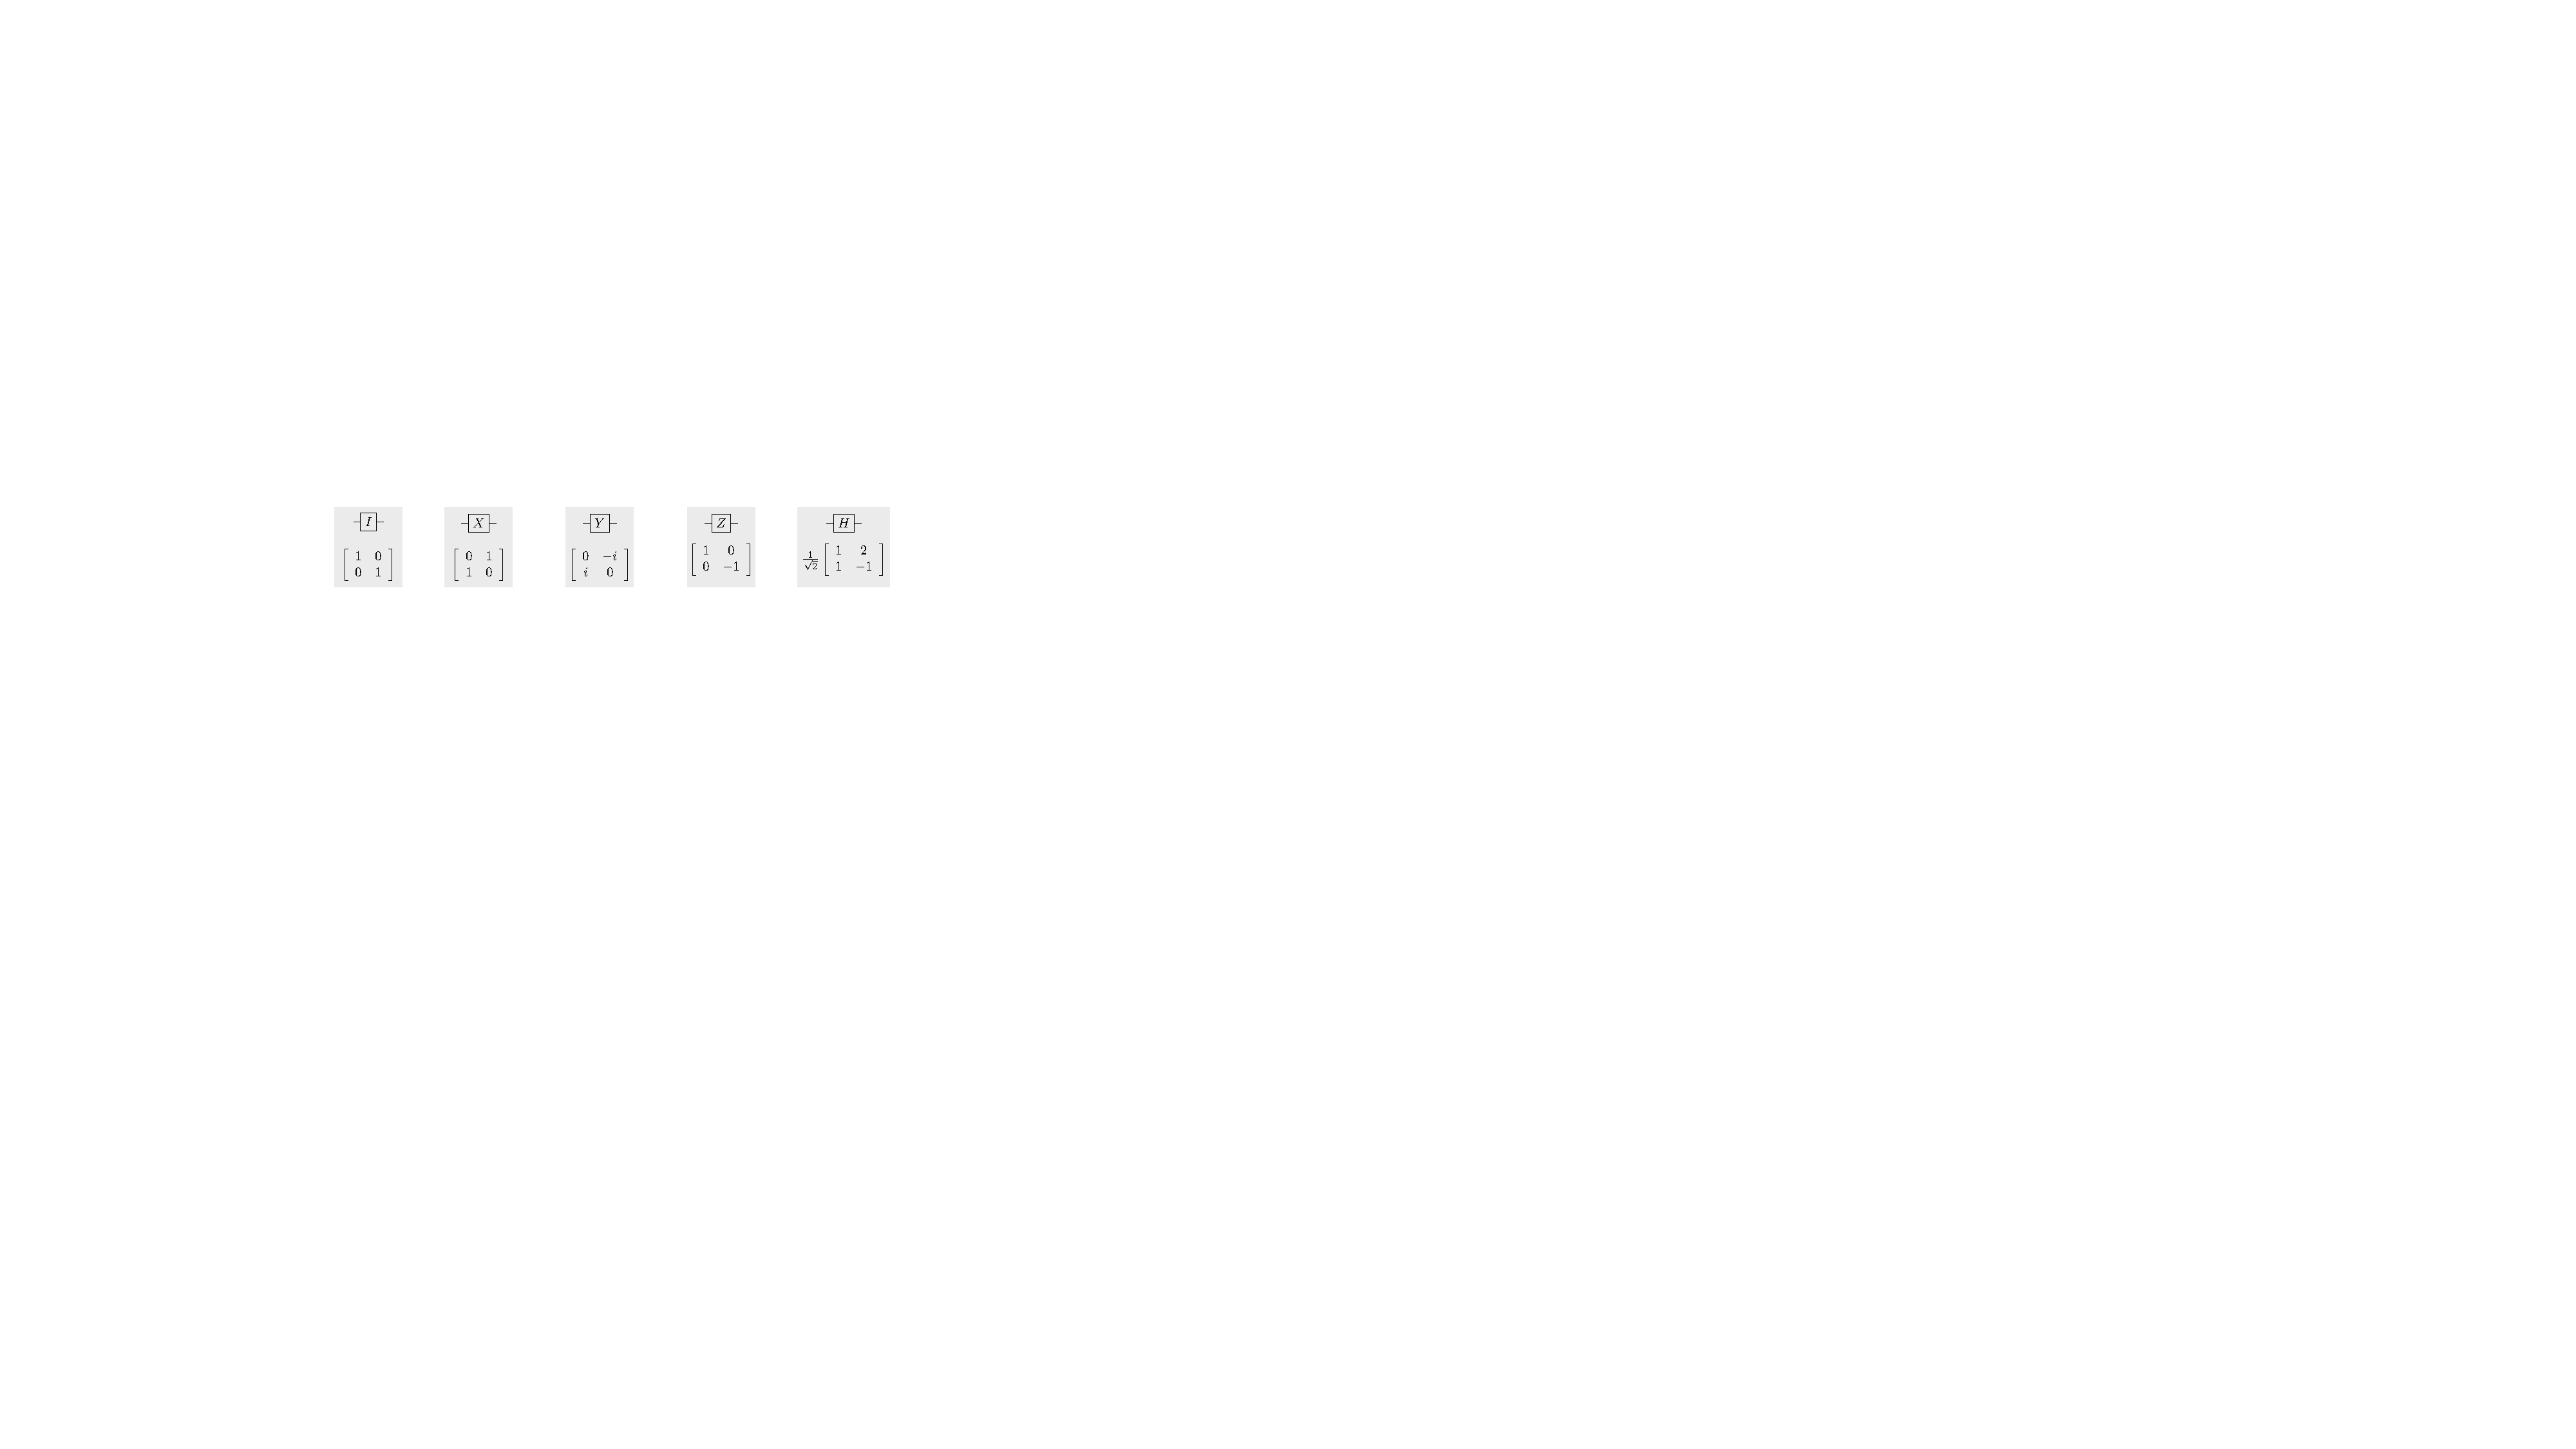
\includegraphics[scale=0.7]{Figures/Gates/qgates} 
\caption{The Identity gate, the Pauli gates, and the Hadamard gate.}
\label{qgates:fig} 
\end{figure}
In a similar manner to classical gates, we will represent quantum gate behaviors by matrices.
%
Quantum gates are {\it reversible}: if we run the gate and then run the inverse of the gate, then we get the identity matrix.
%
Formally, the matrix representing the gate should be {\it unitary}, i.e., its conjugate transpose should be equal to its inverse.
%
In \cref{qgates:fig} we show some examples of quantum gates and their behaviors.
%
The gate $\idgate$ is the identity, and maps each input to an identical output.
%
Next, we introduce the three Pauli gates.

The $\xpgate$ is the quantum analogue of the classical $\notgate$ gate, acting on a single qubit. 
%
It is often referred to as \emph{bit-flip gate} because it inverts the state.
%
In classical computing, a $\notgate$ gate flips a binary value—changing $0$ to $1$ and vice versa. 
%
The $\xpgate$ gate performs the same operation in the quantum domain for the basis states.
%
\[
X\ketof{0} = \ketof{1}\;\;\; \quad X\ketof{1} = \ketof{0}
\]
Moreover, unlike classical bits, qubits can exist in \emph{superpositions} of $\ketof{0}$ and $\ketof{1}$. The $\xpgate$ gate also acts on such states by swapping the amplitudes of the two basis states. For example, consider a qubit in the superposition:
%
\[
\ketof{\psi} = a\ketof{0} + b\ketof{1}
\]
%
where $a$ and $b$ are complex probability amplitudes. Applying the $\xpgate$ gate yields:
%
\[
X\ketof{\psi} = b\ketof{0} + a\ketof{1}
\]
%
Thus, the $\xpgate$ gate exchanges the amplitudes of $\ketof{0}$ and $\ketof{1}$, effectively flipping the qubit's state within the superposition.

The $\zpgate$ gate is also known as the phase-flip gate. 
%
Unlike the $\xpgate$ gate—which acts as a quantum analogue of the classical $\notgate$ gate by flipping the state between $\ketof0$ and $\ketof1$, the $\zpgate$ gate leaves the computational basis states unchanged but inverts the phase of the $\ketof1$ component. In other words, it modifies the relative phase between $\ketof0$ and $\ketof1$, a core concept in quantum mechanics.
%
Thus, applying the $\zpgate$ gate to a qubit in state $\ketof0$ has no effect, while applying it to $\ketof1$ multiplies the state by $-1$, effectively flipping its phase.
%
Due to this nature,  $\zpgate$ is sometimes called phase-flip.
%
This operation is essential in many quantum algorithms and plays a critical role in phase manipulation and interference, which are central to quantum computation.

%
%
The $\ypgate$ gate is a combination of the $\xpgate$ and $\zpgate$ gates, meaning it applies both a bit-flip and a phase-flip to the qubit. 
%
It changes both the state of the qubit (like the $\xpgate$ gate), and the relative phase between the states $\ketof0$ and $\ketof1$ (like the $\zpgate$ gate).

For example, if you have a qubit in the state $\ketof0$ and apply the $\ypgate$ gate, the qubit's state changes to the state $i\ketof1$. 
%
If you have a qubit in the state $\ketof1$ and apply the $\ypgate$ gate, the qubit's state changes to the state $-i\ketof0$.
%
Consider a qubit in the following superposition state:
$\ketof\psi= a\ketof0 + b\ketof1$, where $a$ and $b$ are complex numbers representing the amplitudes of the qubit states.
When the $\ypgate$ gate is applied to this qubit, the result will be:
$Y\ketof\psi = -i b\ketof0 + i a\ketof1$.
%
We observe that the $\ypgate$ gate has not only swapped the amplitudes of the $\ketof0$ and $\ketof1$ states but also added a relative phase of $i$ to the resulting states.

The {\it Hadamard} gate (often denoted as $\hgate$) is a fundamental single-qubit gate in quantum computing. 
%
It creates superposition states, which are essential for quantum parallelism.
%
It transforms the basis states as follows:
\[
\hgate\ketof0=\frac{1}{\sqrt2}(\ketof0+\ketof1)
\;\;\;
\hgate\ketof1=\frac{1}{\sqrt2}(\ketof0-\ketof1)
\]
%
The $\hgate$ gate has three important properties:
\begin{itemize}
\item
{\it Self-inverse}: $\hgate^2 = \idgate$, so applying it twice returns the original state.
\item
Creates superposition: Crucial for quantum algorithms like Deutsch-Jozsa, Grover’s, and Shor’s.
\item
Balanced output: Equal amplitude for both $\ketof0$ and $\ketof1$  (up to a sign), enabling interference.
\end{itemize}

\paragraph{Tree Transformations}

\begin{figure}[ht] 
    \centering
    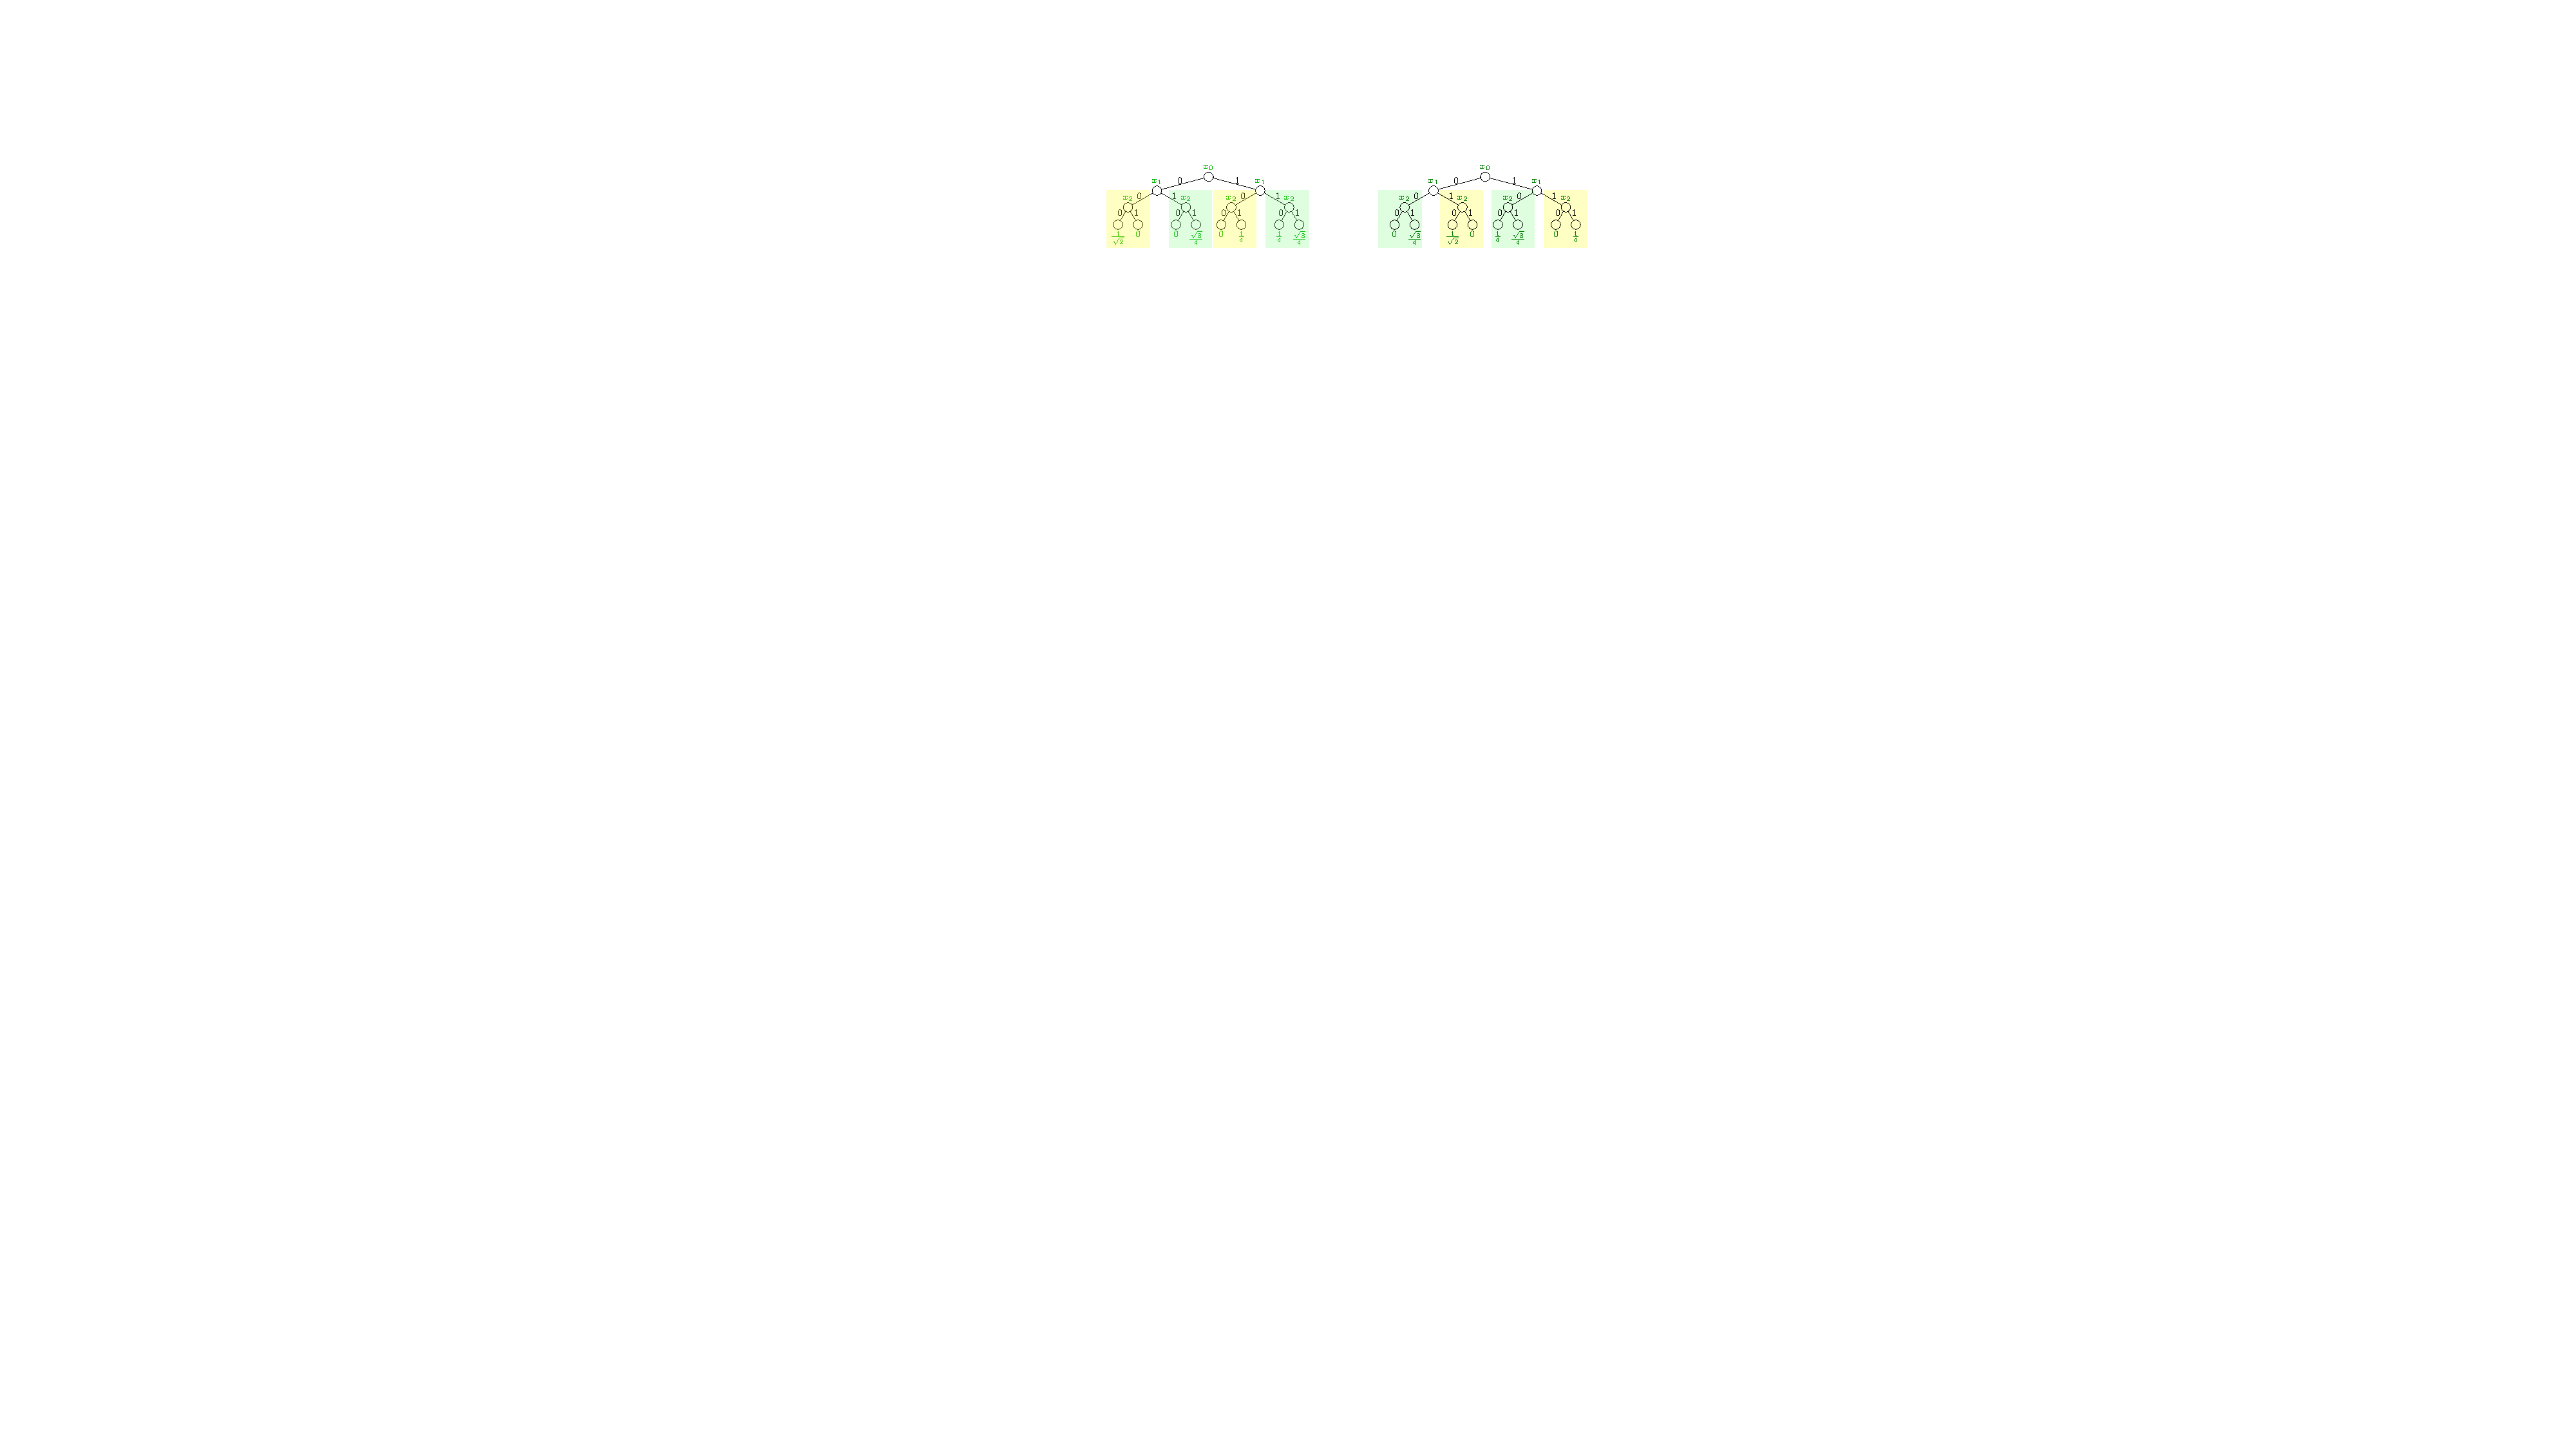
\includegraphics[scale=0.9]{Figures/Trees/ApplyNOT} 
    \caption{Applying the $X$ gate on an input tree. 
    We apply the gate to the bit $\xvar_1$.
    The application is modeled by swapping the left and right subtrees of all nodes at the level corresponding to the qubit $\xvar_1$ (i.e., level~1 in this case).}
    \label{apply:not:fig}
\end{figure}

\begin{figure}[ht] 
    \centering
    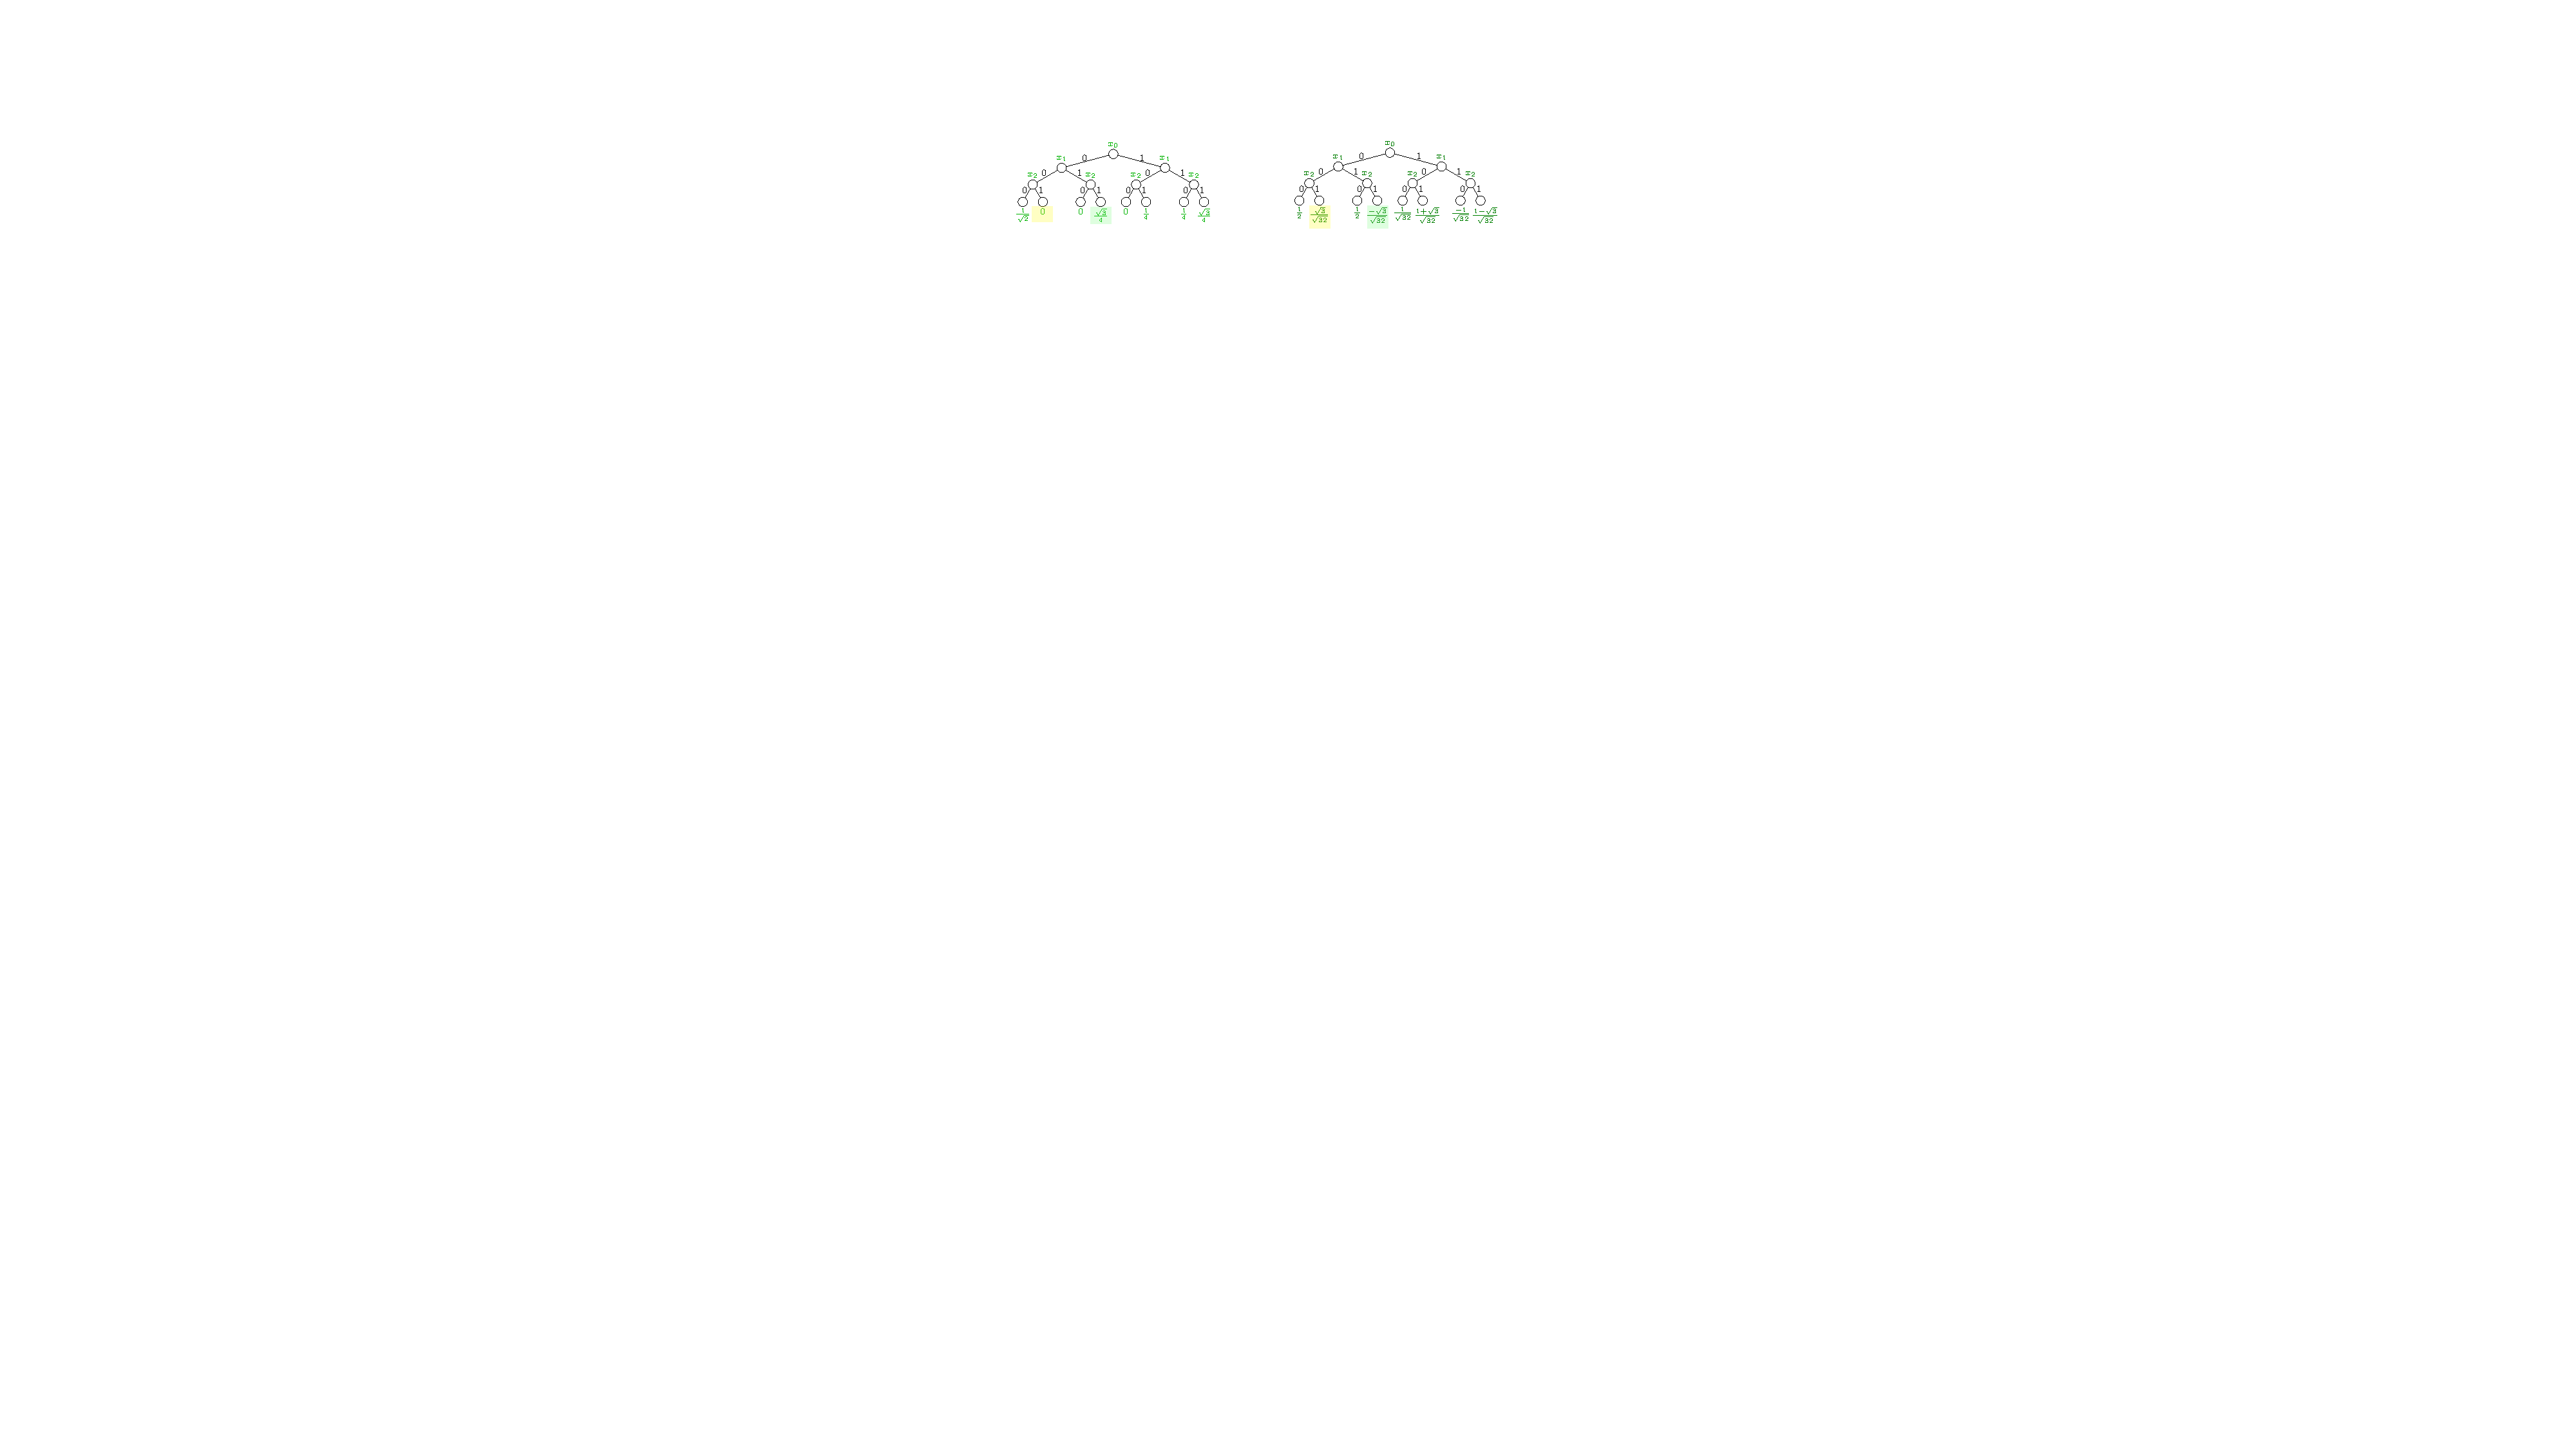
\includegraphics[scale=0.9]{Figures/Trees/ApplyH} 
    \caption{Applying the $\hgate$ gate on an input tree. 
    The gate is applied to the bit $\xvar_1$.
    This transformation also targets all nodes at level~1 (corresponding to $\xvar_1$), updating subtree structure and amplitudes accordingly.}
    \label{apply:H:fig}
\end{figure}

In our setting, we encode gate applications as tree transformations.
Given a tree representing a quantum state, a qubit $\xvar$, and a gate, we compute a new tree that describes the quantum state resulting from applying the gate to the given qubit.

A major difference from the classical setting is that, due to quantum superposition, the effect of a gate application is generally \emph{global}.
That is, we must update all parts of the state in which the qubit $\xvar$ is involved.

In \cref{apply:not:fig} and \cref{apply:H:fig}, we illustrate this by swapping all subtrees at nodes corresponding to $\xvar_1$.
As shown in the example, a gate application can affect the amplitudes of exponentially many leaves—effectively updating an exponential number of classical states.
